\documentclass[11pt]{standalone}
\usepackage{tikz}
\usepackage{pgfplots}
\usepackage{amssymb}
\usepackage{amsmath}
\usepackage{newtxtext,newtxmath}

\usetikzlibrary{shapes.arrows}
\usetikzlibrary{decorations.pathmorphing}
\usetikzlibrary{positioning}
\usetikzlibrary{calc}

\def\widthA{5}
\def\heightA{3}
\def\widthB{5}
\def\heightB{4}

\begin{document}
    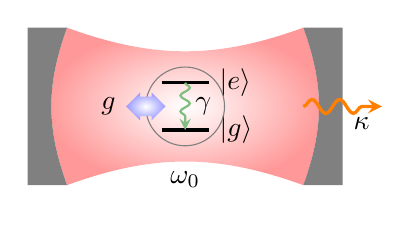
\begin{tikzpicture}
        % \node[anchor=north west, inner sep=0pt] {(a)};
        \begin{scope}[shift={($(\widthA*0.5,-\heightA*0.5)$)}]
            \shade[inner color=white, outer color=red!40] (-1.5, 1) to[bend
            right=20] (1.5, 1) to[bend left=20] (1.5, -1)
            to[bend right=20] node[below]
            {$\omega_0$} (-1.5, -1) to[bend left=20] (-1.5, 1);

            \fill[gray] (-1.5, 1) -- (-2, 1) -- (-2, -1) -- (-1.5, -1) to[bend left=20]
            (-1.5, 1);

            \fill[gray] (1.5, 1) -- (2, 1) -- (2, -1) -- (1.5, -1) to[bend
            right=20]
            (1.5, 1);

            \draw[very thick] (-0.3, 0.3) -- (0.3, 0.3) node[right] {$|e\rangle$};
            \draw[very thick] (-0.3, -0.3) -- (0.3, -0.3) node[right]
            {$|g\rangle$};
            \draw[thin, gray] (0,0) circle (0.5);


            \node[shade, inner color=white, outer color=blue!40,double arrow, 
                  minimum height=5mm, double arrow head extend=1.5,label=left:$g$] at (-0.5,0) {};

            \draw[->,>=stealth,very thick,orange,decorate,decoration={snake,post
            length=1mm}] (1.5, 0) -- (2.5,
            0) node[midway,below right,black] {$\kappa$};

            \draw[->,>=stealth,thick,green!50!black!50,decorate,decoration={snake,
            amplitude=.6mm,segment length=2mm,post length=1mm}] (0, 0.3) --
            (0,-0.3) node[midway,right,black] {$\gamma$};
        \end{scope}
    \end{tikzpicture}
\end{document}
